% Chapter Template

\chapter{Results and Discussion} % Main chapter title

\label{Chapter5} % Change X to a consecutive number; for referencing this chapter elsewhere, use \ref{ChapterX}

%----------------------------------------------------------------------------------------
%	SECTION 1
%----------------------------------------------------------------------------------------

\section{Experiments Description} \label{section:Experiments Description}
Two data sets have been analyzed in this research, ISO New England and ONS data sets. The objective was to evaluate how well the regression models may predict the electricity demand between different machine learning algorithms. In order to achieve highest $R^2$ score for all researched algorithms, an AutoML toolkit has been used to rapid select the best hyper-parameters as explained in \ref{subsection:Automated Machine Learning (AutoML)}.

\subsection{Stationarity Test}
The Augmented Dickey–Fuller (DF) test \citep{dickey_distribution_1979} shows that the both time series are stationary as shown in Table \ref{tab:dickey-fuller}.


\begin{figure}[!htpb]
\centering
\includegraphics[width=1.0\textwidth,height=\textheight,keepaspectratio]{Figures/ACF_demand.pdf}
\caption{ISONewEngland dataset - Autocorrelation Function on Demand Time Series Data}
\label{fig:ISONE_ACF_demand}
\end{figure}

\begin{figure}[!htpb]
\centering
\includegraphics[width=1.0\textwidth,height=\textheight,keepaspectratio]{Figures/ACF_1stdiff.pdf}
\caption{ISONewEngland dataset - Autocorrelation Function on 1st Differencing Demand Time Series Data }
\label{fig:ISONE_ACF_demand_1stdiff}
\end{figure}

\begin{figure}[!htpb]
\centering
\includegraphics[width=1.0\textwidth,height=\textheight,keepaspectratio]{Figures/ACF_1stdiff_zoom.pdf}
\caption{ISONewEngland dataset - Autocorrelation Function on 1st Differencing Demand Time Series Data - lag = 250 }
\label{fig:ISONE_ACF_demand_1stdiff}
\end{figure}



\section{ISO New England data set - Analysis} \label{section:ISO New England data set - Analysis}
In this section, it's shown the results over experiments made on different machine learning algorithms studied in this data set from ISO New England utility. Algorithms covered in this data set are Artificial Neural Networks (ANN), Long Short Term Memory (LSTM), Decision Trees (DT), Random Forests (RF) and Extreme Gradient Boosting (XGBoost).


\subsection{ANN Regression Model} \label{subsection:ANN Regression Model}
First algorithm studied was ANN, which was possible to achieve $R^2$ score over $0.90$ as shown in Table \ref{tab:ANNresults1}. The AutoML NNI has been searched through 7 different parameters, 21 in total as shown in Table \ref{tab:ANNparams}, such as neurons width, hidden layers, different neuron activations, epochs and so on. The experiment ran over 58 hours with 524 trials as shown in Table \ref{tab:ANNresults2}.

Analysing the results, the Table \ref{tab:ANNresults1} shows that batch normalization was inexpressive, also low number of hidden layers show a better response. In addition, neurons width seems to be quite random, where 16 or 128 could achieve a high $R^2$ score anyway. Nevertheless, the duration is not so relevant, since a ANN learning process may last over 6 minutes or under 2 minutes and reach a similar result. Batch size seems quite random as well, it might depend of the combination of hyper-parameters. Last but not least, number of epochs may be optimized by using early stop regularization, since 60 epochs seems to be dominant in top ten results, some 20 epochs appears here as well, so it really depends of combination of parameters.


\begin{table}[!htpb]
\small
\centering
\caption{ANN hyper-parameters used in AutoML}
\label{tab:ANNparams}
% \resizebox{\textwidth}{!}{%
\begin{tabular}{llllll} \hline
\textbf{Hyper-parameter} & \textbf{Values} & \textbf{} &  &  &  \\ \hline
optimizer & Adam &  &  &  &  \\
neurons width & 16 & 32 & 64 & 128 &  \\
hidden layers & 2 & 4 & 8 & 16 & 32 \\
activation & ReLu & LReLU 0.01 & LReLU 0.05 & LReLU 0.1 &  \\
batch normalization & BatchNorm & none &  &  &  \\
batch size & 10 & 20 & 30 &  &  \\
epochs & 20 & 60 &  &  &  \\
\textbf{Total parameters} & \textbf{21} &  &  &  & \\ \hline
\end{tabular}
% }
\end{table}


\begin{table}[!htpb]
\centering
\caption{ANN - Highest ten $R^2$ scores}
\label{tab:ANNresults1}
\resizebox{\textwidth}{!}{%
\begin{tabular}{cccccccccc} \hline
\textbf{id} & \textbf{\begin{tabular}[c]{@{}l@{}}$R^2$\\ score\end{tabular}} & \textbf{\begin{tabular}[c]{@{}l@{}}duration\\ (min)\end{tabular}} & \textbf{optimizer} & \textbf{\begin{tabular}[c]{@{}l@{}}neurons\\ width\end{tabular}} & \textbf{\begin{tabular}[c]{@{}l@{}}hidden\\ layers\end{tabular}} & \textbf{activation} & \textbf{\begin{tabular}[c]{@{}l@{}}batch\\ normalization\end{tabular}} & \textbf{\begin{tabular}[c]{@{}l@{}}batch\\ size\end{tabular}} & \textbf{epochs} \\ \hline
D8ina & 0.9012 & 2.72 & Adam & 16 & 8 & LReLU (0.05) & none & 30 & 60 \\
QmWoh & 0.8996 & 3.67 & Adam & 16 & 8 & LReLU (0.05) & none & 20 & 60 \\
mm6Jz & 0.8993 & 2.68 & Adam & 32 & 8 & ReLu & none & 10 & 20 \\
vaacj & 0.8968 & 6.02 & Adam & 128 & 2 & ReLu & none & 10 & 60 \\
hJ30W & 0.8954 & 2.41 & Adam & 64 & 2 & ReLu & none & 30 & 60 \\
z2ib5 & 0.8944 & 5.71 & Adam & 32 & 4 & LReLU (0.01) & none & 10 & 60 \\
RH5KA & 0.8927 & 3.07 & Adam & 64 & 2 & LReLU (0.01) & none & 20 & 60 \\
Su2hl & 0.8920 & 2.41 & Adam & 32 & 4 & LReLU (0.1) & none & 10 & 20 \\
xroqH & 0.8919 & 1.39 & Adam & 32 & 8 & LReLU (0.01) & none & 30 & 20 \\
VX9dj & 0.8911 & 5.60 & Adam & 64 & 2 & LReLU (0.1) & none & 10 & 60 \\ \hline
\end{tabular}%
}
\end{table}


\begin{table}[!htpb]
\small
\centering
\caption{ANN Experiment Summary}
\label{tab:ANNresults2}
\begin{tabular}{ll} \hline
\textbf{id} & LiNYuulo \\
\textbf{duration (hours)} & 58.86 \\
\textbf{trials} & 524 \\
\textbf{best result} & 0.9012 \\ \hline
\end{tabular}
\end{table}




\subsection{LSTM Regression Model}

LSTM algorithm brings memory feature to the regression model and seems to suffer less to perform through long learning processes on time-series data. However, the results of the model for this study were under performed when compared to the other models. It could only achieve 0.8563 on highest $R^2$ score as shown in Table \ref{tab:LSTMResults1}, which it's not so inferior to the others, but it's disappointing. The AutoML has been searched through 7 different parameters, 24 in total as shown in Table \ref{tab:LSTMResults2}, such as neurons width, hidden layers, different neuron activations, epochs and so on. The experiment ran over 66 hours with 129 trials as shown in Table \ref{tab:LSTMResults3}.

Analysing the LSTM results, the training duration was quite high, which with certain parameters it could ran over 7 hours straight, which does not means it achieved a high $R^2$ score, since a training with half an hour could achieve a better result then, as id Euz1X depicted in Table \ref{tab:LSTMResults1}. About function activations, ReLU and Leaky ReLU are dominant on highest top ten $R^2$ scores, which SeLU and eLU activations were inexpressive on this experiment. In addition, dropout parameter follows the same been not so relevant, since its presence only could affect negatively to the results. Nevertheless, neurons width and hidden layers were fairly diverse but less than 32 neurons would not achieve the greatest results, which is same for more than 16 hidden layers. Last but not least, batch size stick between 12 and 24, which 12 achieved highest $R^2$ scores.


\begin{table}[!htpb]
\centering
\caption{LSTM - Highest ten $R^2$ scores}
\label{tab:LSTMResults1}
\resizebox{\textwidth}{!}{%
\begin{tabular}{lllllllll} \hline
\textbf{id} & \textbf{\begin{tabular}[c]{@{}l@{}}$R^2$\\ score\end{tabular}} & \textbf{\begin{tabular}[c]{@{}l@{}}duration\\ (hours)\end{tabular}} & \textbf{activation} & \textbf{dropout} & \textbf{optimizer} & \textbf{\begin{tabular}[c]{@{}l@{}}neurons\\ width\end{tabular}} & \textbf{\begin{tabular}[c]{@{}l@{}}hidden\\ layers\end{tabular}} & \textbf{\begin{tabular}[c]{@{}l@{}}batch\\ size\end{tabular}} \\ \hline
Fkdx4 & 0.8563 & 2.09 & ReLU & False & Adam & 64 & 8 & 12 \\
AXBYw & 0.8395 & 1.78 & LReLU (0.01) & False & Adam & 32 & 8 & 12 \\
Euz1X & 0.8187 & 0.52 & ReLU & False & Adam & 64 & 16 & 24 \\
l2xSk & 0.8006 & 7.21 & ReLU & False & Adagrad & 128 & 16 & 12 \\
NaSHJ & 0.8002 & 1.38 & LReLU (0.01) & False & Adam & 128 & 2 & 24 \\
OARCU & 0.7956 & 1.71 & LReLU (0.01) & False & Adam & 64 & 2 & 24 \\
JCsde & 0.7851 & 0.95 & LReLU (0.1) & False & Adam & 32 & 16 & 24 \\
Kp8h1 & 0.7812 & 0.90 & LReLU (0.05) & False & Adam & 32 & 16 & 24 \\
WD9gt & 0.7739 & 7.33 & LReLU (0.01) & False & Adagrad & 128 & 16 & 12 \\ \hline
\end{tabular}%
}
\end{table}

\begin{table}[!htpb]
\small
\centering
\caption{LSTM hyper-parameters used in AutoML}
\label{tab:LSTMResults2}
% \resizebox{\textwidth}{!}{%
\begin{tabular}{ccccccc} \hline
\textbf{Hyper-parameters} & \textbf{Values} &  &  &  &  &  \\ \hline
\textbf{optimizer} & Adam & RMSProp & Adagrad & Adadelta &  &  \\
\textbf{neurons\_width} & 16 & 32 & 64 & 128 &  &  \\
\textbf{hidden\_layers} & 2 & 4 & 8 & 16 &  &  \\
\textbf{activation} & SELU & ELU & ReLU & \begin{tabular}[c]{@{}l@{}}Leaky\\ ReLU (0.01)\end{tabular} & \begin{tabular}[c]{@{}l@{}}Leaky\\ ReLU (0.05)\end{tabular} & \begin{tabular}[c]{@{}l@{}}Leaky\\ ReLU (0.1)\end{tabular} \\
\textbf{batch\_size} & 12 & 24 & 48 & 72 &  &  \\
\textbf{dropout (0.2)} & True & False &  &  &  &  \\ \hline
\textbf{Total parameters} & 24 &  &  &  &  & \\ \hline
\end{tabular}
% }
\end{table}

\begin{table}[!htpb]
\small
\centering
\caption{LSTM - Experiment Summary}
\label{tab:LSTMResults3}
\begin{tabular}{ll} \hline
\textbf{id} & kBlhC0PA \\
\textbf{duration (hours)} & 66.70 \\
\textbf{trials} & 129 \\
\textbf{best result} & 0.8563 \\ \hline
\end{tabular}
\end{table}


\subsection{Random Forest Model}



\begin{table}[!htpb]
\centering
\caption{Random Forest - Highest ten $R^2$ scores}
\label{tab:RFResults1}
\resizebox{\textwidth}{!}{%
\begin{tabular}{lllllllllll} \hline
\textbf{id} & \textbf{\begin{tabular}[c]{@{}l@{}}$R^2$\\ score\end{tabular}} & \textbf{duration (s)} & \textbf{\begin{tabular}[c]{@{}l@{}}max\\ features\end{tabular}} & \textbf{\begin{tabular}[c]{@{}l@{}}max\\ leaf\\ nodes\end{tabular}} & \textbf{\begin{tabular}[c]{@{}l@{}}min\\ samples\\ leaf\end{tabular}} & \textbf{estimators} & \textbf{\begin{tabular}[c]{@{}l@{}}min\\ samples\\ split\end{tabular}} & \textbf{\begin{tabular}[c]{@{}l@{}}min\\ impurity\\ decrease\end{tabular}} & \textbf{\begin{tabular}[c]{@{}l@{}}max\\ depth\end{tabular}} & \textbf{bootstrap} \\ \hline
yF4G2 & 0.9526 & 66.9 & auto & None & 1 & 750 & 2 & 0.001 & 32 & True \\
E3Yt3 & 0.9526 & 77.4 & auto & None & 1 & 750 & 2 & 0.001 & 128 & True \\
z6pAq & 0.9526 & 64.9 & auto & None & 1 & 750 & 2 & 0.1 & 32 & True \\
DcaFJ & 0.9526 & 71.3 & auto & None & 1 & 750 & 2 & 0.1 & 128 & True \\
aeh4D & 0.9526 & 69.2 & auto & None & 1 & 750 & 2 & 0.1 & 256 & True \\
NrgwK & 0.9526 & 64.9 & auto & None & 1 & 750 & 2 & 0.1 & 64 & True \\
DIzMv & 0.9526 & 63.1 & auto & None & 1 & 750 & 4 & 0.1 & 128 & True \\
pTskN & 0.9526 & 52.4 & auto & None & 1 & 750 & 4 & 0.001 & 256 & True \\
muBKm & 0.9525 & 52.6 & auto & None & 1 & 500 & 2 & 0.001 & 64 & True \\
cOeNA & 0.9524 & 30.3 & auto & None & 1 & 250 & 2 & 0 & 256 & True \\ \hline
\end{tabular}%
}
\end{table}



\begin{table}[!htpb]
\small
\centering
\caption{Random Forest hyper-parameters used in AutoML}
\label{tab:RFResults2}
\begin{tabular}{lllllll} \hline
\textbf{Hyper-parameters} & \textbf{Values} &  &  &  &  &  \\ \hline
max\_features & auto & sqrt & log2 &  &  &  \\
max\_leaf\_nodes & 8 & 16 & 32 & 64 & 128 & 256 \\
min\_samples\_leaf & 1 & 2 & 4 & 8 & 16 & 32 \\
n\_estimators & 100 & 250 & 500 & 750 & 1000 &  \\
min\_samples\_split & 2 & 4 & 8 & 16 & 32 &  \\
min\_impurity\_decrease & 0 & 0.001 & 0.01 & 0.05 & 0.1 &  \\
max\_depth & 16 & 32 & 64 & 128 & 256 &  \\
bootstrap & False & True &  &  &  &  \\ \hline
\textbf{Total parameters} & \textbf{37} &  &  &  &  & \\ \hline
\end{tabular}
\end{table}


\begin{table}[!htpb]
\small
\centering
\caption{Random Forest - Experiment Summary}
\label{tab:RFResults3}
\begin{tabular}{ll} \hline
\textbf{id} & konggImF \\
\textbf{duration (hours)} & 16.47 \\
\textbf{trials} & 2000 \\
\textbf{best result} & 0.9526 \\ \hline
\end{tabular}
\end{table}


\subsection{XGBoost Regression Model}
XGBoost is known as fast ensemble method, which rapidly can be implemented and tested without many setup and configuration. With this algorithm, it was possible to achieve $R^2$ score over $0.96$ as shown in Table \ref{tab:XGBoostResults2}, also other nine highest outputs are shown in the same table. NNI has been searched through 9 different hyper-parameters, in total 34 as shown in Table \ref{tab:XGBoostParams}, such as learning rate, number of estimators, subsample, max depth and so on. This experiment ran over 23.5 hours, with 658 trials as shown in \ref{tab:XGBoostResults3}.

The results are expressive, the highest ten $R^2$ scores are above 0.96, which makes this model very accurate in predicting time-series electricity demand for ISO New England dataset. The \textit{duration} of trials were between 1 minute and 6 minutes. The \textit{subsample} parameter tends to 0.1 than 0.6, \textit{maximum depth} varies between 5 and 12, which 3 seems too shallow to get highest results. \textit{Learning rate} lower is better, set as 0.001, maybe even less could output superior scores. The \textit{number of estimators} are quite random, but overall 1000 is a reasonable choice. The parameter \textit{gamma} is not so dominant in one value, it probably depends from other hyper-parameters, which is the opposite of \textit{colsample bytree} where 0.8 is the regular value. \textit{Reg lambda} and \textit{reg alpha} are not so easy to read, which seems quite random. For \textit{min child weight} parameter mainly lower values seems better, as 1.5 value corresponds to it. 




\begin{table}[!htpb]
\small
\centering
\caption{XGBoost - Hyper-parameters used in AutoML}
\label{tab:XGBoostParams}
\begin{tabular}{llllll} \hline
\textbf{Hyper-parameter} & \textbf{Values} & \textbf{} & \textbf{} & \textbf{} & \textbf{} \\ \hline
colsample\_bytree & 0.4 & 0.6 & 0.8 &  &  \\
gamma & 0 & 0.03 & 0.10 & 0.30 & 0.70 \\
learning\_rate & 0.1 & 0.05 & 0.01 & 0.001 &  \\
max\_depth & 3 & 5 & 7 & 12 &  \\
min\_child\_weight & 1.5 & 6 & 10 &  &  \\
n\_estimators & 500 & 1000 & 2000 & 4000 &  \\
reg\_alpha & 1e-5 & 0.01 & 0.75 & 1 &  \\
reg\_lambda & 1e-5 & 0.01 & 0.45 & 1 &  \\
subsample & 0.10 & 0.60 & 0.95 &  &  \\ \hline
\textbf{Total parameters} & \textbf{34} &  &  &  & \\ \hline
\end{tabular}
\end{table}


\begin{table}[!htpb]
\small
\centering
\caption{XGBoost Experiment Summary}
\label{tab:XGBoostResults3}
\begin{tabular}{ll} \hline
\textbf{id} & XpOLJXtn \\
\textbf{duration (hours)} & 23.51667 \\
\textbf{trials} & 658 \\
\textbf{best result} & 0.961943 \\ \hline
\end{tabular}
\end{table}


\begin{table}[!htpb]
\centering
\caption{XGBoost - Highest ten $R^2$ scores}
\label{tab:XGBoostResults2}
\resizebox{\textwidth}{!}{%
\begin{tabular}{cccccccccccc} \hline
\textbf{id} & \textbf{\begin{tabular}[c]{@{}l@{}}duration\\ (min)\end{tabular}} & \textbf{\begin{tabular}[c]{@{}l@{}}$R^2$\\ score\end{tabular}} & \textbf{subsample} & \textbf{\begin{tabular}[c]{@{}l@{}}max\\ depth\end{tabular}} & \textbf{\begin{tabular}[c]{@{}l@{}}learning\\ rate\end{tabular}} & \textbf{\begin{tabular}[c]{@{}l@{}}number of\\ estimators\end{tabular}} & \textbf{gamma} & \textbf{\begin{tabular}[c]{@{}l@{}}colsample\\ bytree\end{tabular}} & \textbf{\begin{tabular}[c]{@{}l@{}}reg\\ lambda\end{tabular}} & \textbf{\begin{tabular}[c]{@{}l@{}}min child\\ weight\end{tabular}} & \textbf{\begin{tabular}[c]{@{}l@{}}reg\\ alpha\end{tabular}} \\ \hline
zihIV & 1.46 & 0.9619 & 0.1 & 12 & 0.01 & 1000 & 0.70 & 0.8 & 0.45 & 1.5 & 1.00 \\
fixzE & 1.47 & 0.9619 & 0.1 & 12 & 0.01 & 1000 & 0.03 & 0.8 & 0.45 & 1.5 & 0.01 \\
VqFpm & 0.59 & 0.9613 & 0.1 & 5 & 0.05 & 500 & 0.00 & 0.8 & 0.45 & 1.5 & 1e-5 \\
gfzss & 0.94 & 0.9609 & 0.1 & 7 & 0.01 & 1000 & 0.03 & 0.8 & 0.45 & 1.5 & 0.01 \\
NnXKQ & 1.86 & 0.9607 & 0.6 & 12 & 0.01 & 1000 & 0.30 & 0.8 & 1.00 & 10.0 & 0.01 \\
wsSNB & 0.96 & 0.9605 & 0.1 & 7 & 0.01 & 1000 & 0.10 & 0.8 & 0.01 & 1.5 & 0.01 \\
SC0Ps & 1.01 & 0.9605 & 0.1 & 7 & 0.01 & 1000 & 0.03 & 0.8 & 0.01 & 1.5 & 0.01 \\
bo2US & 5.70 & 0.9604 & 0.1 & 12 & 0.01 & 4000 & 0.10 & 0.8 & 1.00 & 1.5 & 1.00 \\
aONKG & 4.18 & 0.9602 & 0.6 & 12 & 0.01 & 2000 & 0.10 & 0.8 & 1.00 & 1.5 & 0.75 \\
qcdIG & 3.75 & 0.9601 & 0.6 & 12 & 0.01 & 2000 & 0.30 & 0.8 & 1.00 & 1.5 & 1.00 \\ \hline
\end{tabular}%
}
\end{table}

\subsection{ISO New England results using EMD}
The results for load forecasting using EMD decomposition is shown in Tables \ref{tab:results_emd_40-fold_1day_part1}, \ref{tab:results_emd_40-fold_1day_part2}, \ref{tab:results_emd_40-fold_1day_part3} and \ref{tab:results_emd_test_set_1d_ahead}. Because of Box-Cox re-scaling, the error metrics for RMSE, MAE, MAPE and sMAPE were misleading, mainly due to numbers near to zero and the scale is different for every IMF generated. Instead, it's better to analyze $R^2$ test metric to compare how well the model predicted the validation set, which surprisingly the composed result in Table \ref{tab:results_emd_40-fold_1day_part3} was way better than the decomposed ones, Tables \ref{tab:results_emd_40-fold_1day_part1}, \ref{tab:results_emd_40-fold_1day_part2}. Comparing with the \textit{No decomposition} method, the EMD method is still behind in all error metrics, but close if compare only MAPE and sMAPE metrics. Then the Table \ref{tab:results_emd_test_set_1d_ahead} shows the forecast results using a test set (unseen values), which EMD method outcomes the \textit{No decomposition} method by far, as MAPE is around $1.92\%$ versus $3.50\%$.

The test set is composed by 24 hourly load values which have not been seen by the model, which are completely new values that have been predicted. 

% Please add the following required packages to your document preamble:
% \usepackage{graphicx}
\begin{table}[!htpb]
\centering
\caption{ISO New England dataset - Load forecasting results using EMD method with 40-fold cross-validation - Part 1.}
\label{tab:results_emd_40-fold_1day_part1}
\resizebox{\textwidth}{!}{%
\begin{tabular}{lrrrr}
\hline
\multicolumn{1}{c}{\textbf{Error metrics}} & \multicolumn{1}{c}{\textbf{IMF\_0}} & \multicolumn{1}{c}{\textbf{IMF\_1}} & \multicolumn{1}{c}{\textbf{IMF\_2}} & \multicolumn{1}{c}{\textbf{IMF\_3}} \\ \hline
\textbf{$R^2$ train} & 0.8695 (+- 0.09) & 0.9429 (+- 0.03) & 0.8679 (+- 0.06) & 0.9215 (+- 0.03) \\
\textbf{$R^2$ test} & 0.3795 (+- 1.20) & 0.1984 (+- 3.72) & -4.1867 (+- 10.02) & -50.1421 (+- 221.21) \\
\textbf{RMSE} & 0.0086 (+- 0.01) & 0.0178 (+- 0.01) & 0.0163 (+- 0.01) & 0.0120 (+- 0.01) \\
\textbf{MAE} & 0.0072 (+- 0.01) & 0.0151 (+- 0.01) & 0.0142 (+- 0.01) & 0.0109 (+- 0.01) \\
\textbf{MAPE} & 411.49 (+- 763.25) & 318.76 (+- 502.31) & 326.26 (+- 245.69) & 312.25 (+- 291.48) \\
\textbf{sMAPE} & 137.37 (+- 12.31) & 137.03 (+- 8.08) & 147.21 (+- 15.68) & 131.17 (+- 35.33) \\ \hline
\end{tabular}%
}
\end{table}



\begin{table}[!htpb]
\centering
\caption{ISO New England dataset - Load forecasting results using EMD method with 40-fold cross-validation - Part 2.}
\label{tab:results_emd_40-fold_1day_part2}
\resizebox{0.85\width}{!}{%
\begin{tabular}{lrrr}
\hline
\multicolumn{1}{c}{\textbf{Error metrics}} & \multicolumn{1}{c}{\textbf{IMF\_4}} & \multicolumn{1}{c}{\textbf{IMF\_5}} & \multicolumn{1}{c}{\textbf{IMF\_6}} \\ \hline
\textbf{$R^2$ train} & 0.9689 (+- 0.02) & 0.9919 (+- 0.00) & 0.9992 (+- 0.00) \\
\textbf{$R^2$ test} & -22.1311 (+- 30.28) & -1453 (+- 8696) & -37.3569 (+- 72.74) \\
\textbf{RMSE} & 0.0116 (+- 0.01) & 0.0086 (+- 0.01) & 0.0040 (+- 0.01) \\
\textbf{MAE} & 0.0109 (+- 0.01) & 0.0082 (+- 0.01) & 0.0039 (+- 0.01) \\
\textbf{MAPE} & 186.46 (+- 258.47) & 126.24 (+- 204.58) & 0.0645 (+- 0.08) \\
\textbf{sMAPE} & 117.78 (+- 63.95) & 86.42 (+- 60.30) & 0.0645 (+- 0.08) \\ \hline
\end{tabular}%
}
\end{table}


\begin{table}[]
\centering
\caption{ISO New England dataset - Load forecasting results using EMD and no decomposition methods with 40-fold cross-validation.}
\label{tab:results_emd_40-fold_1day_part3}
\resizebox{0.65\textwidth}{!}{%
\begin{tabular}{lrr}
\hline
\textbf{Error metrics} & \multicolumn{1}{c}{\textbf{EMD}} & \multicolumn{1}{c}{\textbf{No decomposition}} \\ \hline
\textbf{$R^2$ test} & 0.8625 (+- 0.21) & 0.9101 (+- 0.10) \\
\textbf{RMSE} & 627.26 (+- 380.02) & 541.18 (+- 242.95) \\
\textbf{MAE} & 531.11 (+- 339.57) & 451.84 (+- 208.91) \\
\textbf{MAPE} & 3.7127 (+- 2.27) & 3.177 (+- 1.30) \\
\textbf{sMAPE} & 3.7459 (+- 2.37) & 3.152 (+- 1.26) \\ \hline
\end{tabular}%
}
\end{table}



\begin{table}[]
\centering
\caption{ISO New England dataset - Load forecasting results comparing EMD and no decomposition methods - 1 day ahead forecast - test set.}
\label{tab:results_emd_test_set_1d_ahead}
\resizebox{0.5\textwidth}{!}{%
\begin{tabular}{lcc}
\hline
\multicolumn{3}{c}{\textbf{\begin{tabular}[c]{@{}c@{}}Forecast 1 day ahead\\ Test set\end{tabular}}} \\ \hline
\multicolumn{1}{c}{\textbf{Error metrics}} & \textbf{EMD} & \textbf{No decomposition} \\ \hline
\textbf{$R^2$ train} & 0.958 & 0.863 \\
\textbf{$R^2$ test} & 0.931 & 0.775 \\
\textbf{RMSE} & 306.66 & 553.09 \\
\textbf{MAE} & 249.72 & 462.14 \\
\textbf{MAPE} & 1.92 & 3.50 \\
\textbf{sMAPE} & 1.91 & 3.42 \\ \hline
\end{tabular}%
}
\end{table}



%%%%%%%%%%%%%%%%%%%%
% ONS dataset
%%%%%%%%%%%%%%%%%%%%


\section{ONS data set - Analysis}

In this section, it's shown the results over experiments made on different machine learning algorithms studied in this data set from ONS (\emph{Operador Nacional do Sistema Elétrico} - National Operator of Electric System). Algorithms covered in this data set are Artificial Neural Networks (ANN), Long Short Term Memory (LSTM), Decision Trees (DT), Random Forests (RF) and Extreme Gradient Boosting (XGBoost).


\subsection{ANN Regression Model} \label{subsection:ANN Regression Model - ONS}
The first algorithm to be analyzed on ONS data set analysis is ANN, which could achieve a $R^2$ score over 0.767, not so high than expected. Starting with duration, it seems to take less time when \textit{LeakyReLU} activation is present, in comparison with \textit{ReLU} activation, where 21.5 minutes was the fastest among the highest scores, in contrast 143.7 minutes was needed to finish the slowest one as shown in Table \ref{tab:ONSANNtopten_1}.
LeakyReLU have been the best choice, at the same time Adam optimizer is far better than the others. As have been observed before, dropout parameter does not seem relevant or significantly important to the model. Neurons width are between 32 and 128, where 64 and 128 are more frequent in highest $R^2$ scores. Hidden layers are between 4 and 8, which seems a reasonable number, since there are not so many features to be identified in the data. Last but not least, batch size equals to 24 is the right choice, but others can also be considered in the model parameterization.




\begin{table}[!htpb]
\small
\centering
\caption{ONS Analysis - ANN Experiment Summary}
\label{tab:ONSANN_summary}
\begin{tabular}{ll} \hline
\textbf{Experiment summary} & \textbf{Values} \\ \hline
\textbf{id}                 & QBNIE1bj        \\
\textbf{duration (hours)}   & 65.75           \\
\textbf{trials}             & 512             \\
\textbf{best result}        & 0.7672         \\ \hline
\end{tabular}
\end{table}



\begin{table}[!htpb]
\centering
\caption{ANN - Highest ten $R^2$ scores}
\label{tab:ONSANNtopten_1}
\resizebox{\textwidth}{!}{%
\begin{tabular}{ccccccccc} \hline
\textbf{id} &
  \textbf{\begin{tabular}[c]{@{}l@{}}$R^2$\\ score\end{tabular}} &
  \textbf{\begin{tabular}[c]{@{}l@{}}duration\\ (min)\end{tabular}} &
  \textbf{activation} &
  \textbf{dropout} &
  \textbf{optimizer} &
  \textbf{\begin{tabular}[c]{@{}l@{}}neurons\\ width\end{tabular}} &
  \textbf{\begin{tabular}[c]{@{}l@{}}hidden\\ layers\end{tabular}} &
  \textbf{\begin{tabular}[c]{@{}l@{}}batch\\ size\end{tabular}} \\ \hline
ac5ax & 0.7672 & 32.5   & LReLU (0.05) & False & Adam & 64  & 8 & 24 \\
aAsC6 & 0.7647 & 30.46  & LReLU (0.1) & False & Adam & 128 & 4 & 24 \\
JAoZR & 0.7563 & 21.51  & LReLU (0.1) & False & Adam & 64  & 8 & 24 \\
vpeAz & 0.7555 & 48.32  & LReLU (0.1) & False & Adam & 32  & 8 & 24 \\
zWR1q & 0.7501 & 41.5   & LReLU (0.05) & False & Adam & 64  & 4 & 24 \\
vpP1o & 0.7489 & 39.59  & LReLU (0.05) & False & Adam & 128 & 8 & 24 \\
TsZtS & 0.7486 & 143.74 & relu            & False & Adam & 128 & 4 & 6  \\
WGaXo & 0.7348 & 38.11  & LReLU (0.01) & False & Adam & 32  & 4 & 12 \\
LgV34 & 0.7343 & 53.49  & selu            & False & Adam & 64  & 4 & 24 \\
yeuk3 & 0.7307 & 126.37 & relu            & False & Adam & 64  & 4 & 6 \\ \hline
\end{tabular}%
}
\end{table}


\begin{table}[!htpb]
\small
\centering
\caption{ONS Analysis - ANN Experiment Summary}
\label{tab:ONSANN_summary}
\begin{tabular}{ll} \hline
\textbf{Experiment summary} & \textbf{Values} \\ \hline
\textbf{id}                 & QBNIE1bj        \\
\textbf{duration (hours)}   & 65.75           \\
\textbf{trials}             & 512             \\
\textbf{best result}        & 0.7672         \\ \hline
\end{tabular}
\end{table}


\subsection{XGBoost Regression Model} \label{subsection:XGBoost Regression Model}


\begin{table}[!htpb]
\centering
\caption{XGBoost - Highest ten $R^2$ scores}
\label{tab:XGBoostResultsONStopten}
\resizebox{\textwidth}{!}{%
\begin{tabular}{cccccccccccc}
\hline
\textbf{id} & \textbf{\begin{tabular}[c]{@{}c@{}}duration\\ (min)\end{tabular}} & \textbf{\begin{tabular}[c]{@{}c@{}}$R^2$\\ score\end{tabular}} & \textbf{subsample} & \textbf{\begin{tabular}[c]{@{}c@{}}max\\ depth\end{tabular}} & \textbf{\begin{tabular}[c]{@{}c@{}}learning\\ rate\end{tabular}} & \textbf{\begin{tabular}[c]{@{}c@{}}number of\\ estimators\end{tabular}} & \textbf{gamma} & \textbf{\begin{tabular}[c]{@{}c@{}}colsample\\ bytree\end{tabular}} & \textbf{\begin{tabular}[c]{@{}c@{}}reg\\ lambda\end{tabular}} & \textbf{\begin{tabular}[c]{@{}c@{}}min child\\ weight\end{tabular}} & \textbf{\begin{tabular}[c]{@{}c@{}}reg\\ alpha\end{tabular}} \\ \hline
AAwFn & 1.33 & 0.903 & 0.95 & 5 & 0.01 & 2000 & 0.03 & 0.6 & 1 & 1.5 & 1.00 \\
i6R55 & 1.36 & 0.9028 & 0.1 & 5 & 0.01 & 2000 & 0 & 0.8 & 1 & 1.5 & 1e-5 \\
GpPWn & 1.64 & 0.9028 & 0.1 & 5 & 0.01 & 2000 & 0 & 0.8 & 1 & 1.5 & 0.01 \\
Qwimd & 0.91 & 0.9028 & 0.6 & 7 & 0.01 & 1000 & 0.3 & 0.8 & 1 & 1.5 & 1e-5 \\
iD0g7 & 1.31 & 0.9027 & 0.1 & 5 & 0.01 & 2000 & 0 & 0.8 & 1 & 1.5 & 1.00 \\
Wna6q & 1.43 & 0.9027 & 0.1 & 5 & 0.01 & 2000 & 0 & 0.8 & 1 & 1.5 & 0.75 \\
oxaEo & 1.23 & 0.9025 & 0.6 & 5 & 0.01 & 2000 & 0 & 0.8 & 1e-5 & 10 & 1e-5 \\
ZItlf & 1.29 & 0.9024 & 0.1 & 5 & 0.01 & 2000 & 0 & 0.8 & 1 & 6 & 0.75 \\
Wsi0d & 0.63 & 0.9024 & 0.6 & 5 & 0.05 & 500 & 0.1 & 0.6 & 0.01 & 1.5 & 0.75 \\
yoZG7 & 1.73 & 0.9024 & 0.6 & 5 & 0.01 & 2000 & 0.1 & 0.8 & 0.01 & 10 & 1e-5 \\ \hline
\end{tabular}%
}
\end{table}

\begin{table}[!htpb]
\small
\centering
\caption{ONS Analysis - XGBoost Experiment Summary}
\label{tab:XGBoostResultsONS}
\begin{tabular}{ll}
\hline
\textbf{Experiment summary} & \textbf{Values} \\ \hline
\textbf{id} & Jdtm7v7G \\
\textbf{duration (hours)} & 36.53 \\
\textbf{trials} & 2264 \\
\textbf{best result} & 0.902956 \\ \hline
\end{tabular}
\end{table}




\begin{figure}[!htpb]
\centering
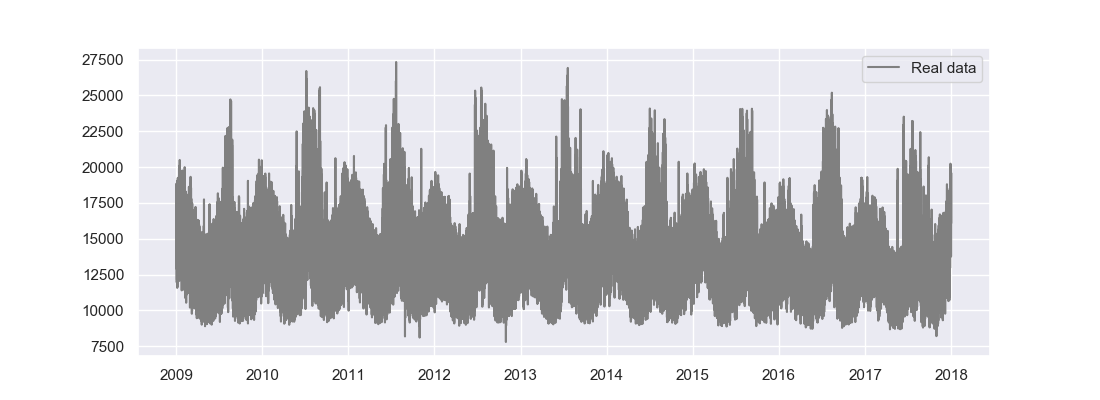
\includegraphics[width=1.0\textwidth,height=\textheight,keepaspectratio]{Figures/Actual_Data.png}
\caption{ISO New England - Demand between 2009 and 2017}
\label{figDemand1}
\end{figure}


\begin{figure}[!htpb]
\centering
\includesvg[width=1.0\textwidth,height=\textheight,keepaspectratio]{Figures/ONS_decompose_additive.svg}
\caption{ONS dataset - Series decomposition over real demand data}
\label{figSeasonD2}
\end{figure}



\begin{figure}[!htpb]
\centering
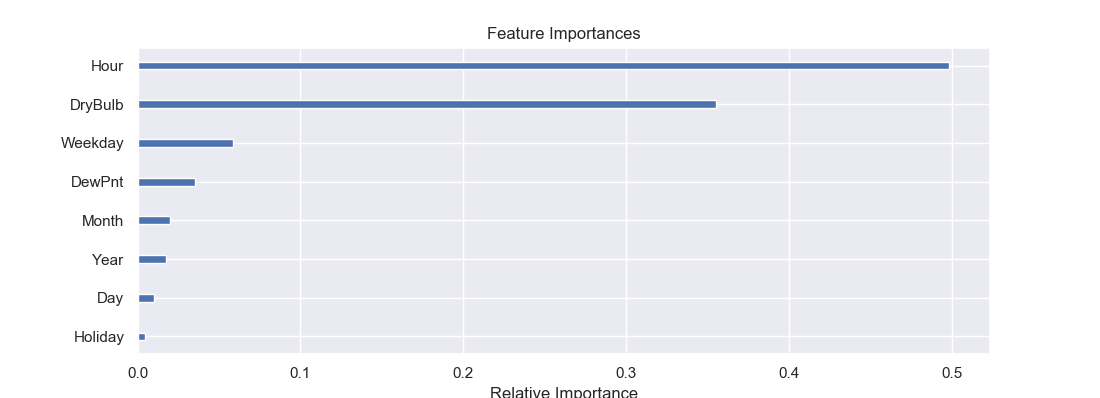
\includegraphics[width=1.0\textwidth,height=\textheight,keepaspectratio]{Figures/Feature_Importance_RF.png}
\caption{Feature importance by Random Forest}
\label{figFeatImp1}
\end{figure}


\begin{figure}[!htpb]
\centering
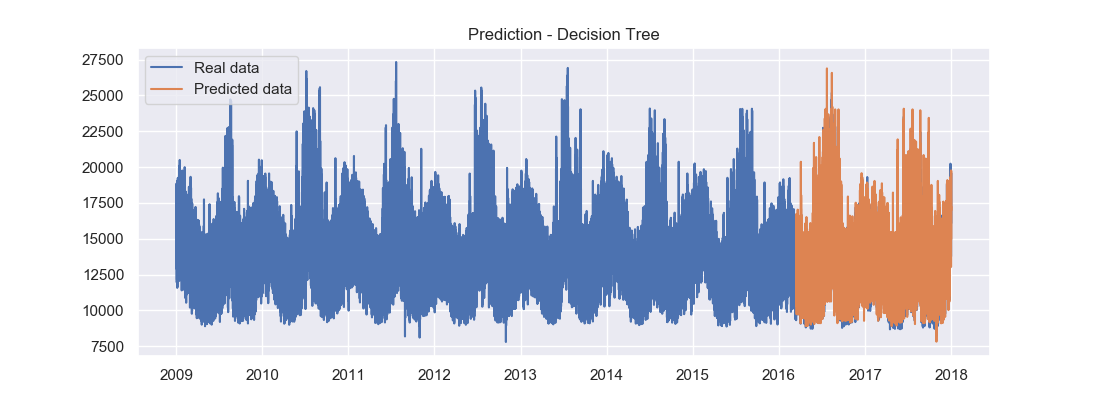
\includegraphics[width=1.0\textwidth,height=\textheight,keepaspectratio]{Figures/DecisionTree_pred.png}
\caption{Prediction of Decision Tree over real demand data}
\label{figDecisionTree1}
\end{figure}


\begin{figure}[!htpb]
\centering
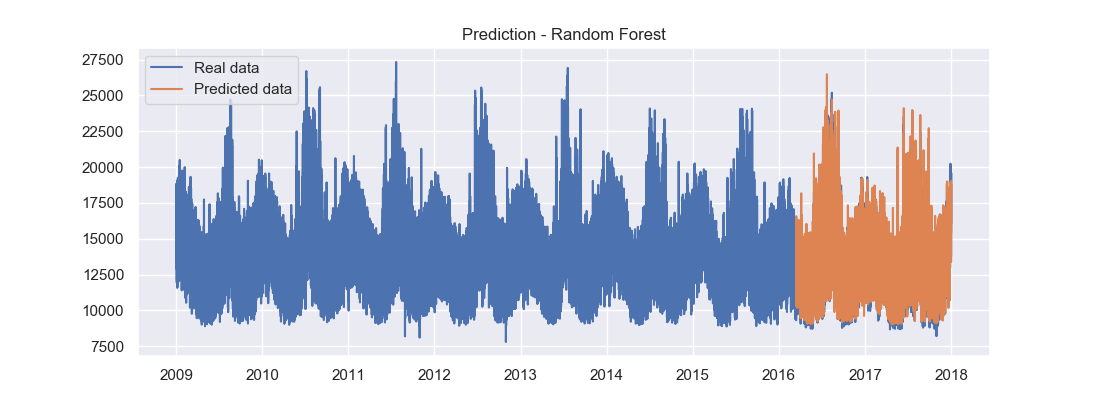
\includegraphics[width=1.0\textwidth,height=\textheight,keepaspectratio]{Figures/RandomForest_pred.png}
\caption{Prediction of Random Forest over real demand data}
\label{figRandForest1}
\end{figure}



\begin{figure}[!htpb]
\centering
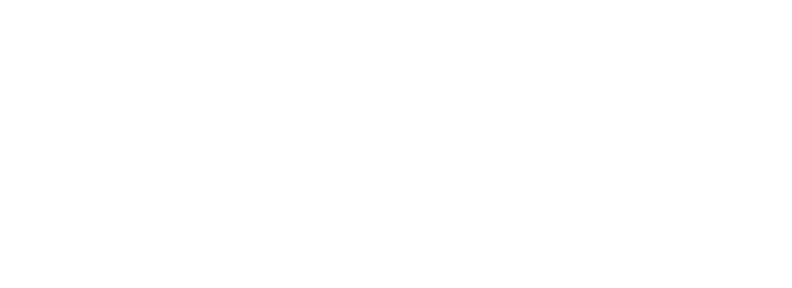
\includegraphics[width=1.0\textwidth,height=\textheight,keepaspectratio]{Figures/XGBoost_pred.png}
\caption{Prediction of XGBoost over real demand data}
\label{figXGB1}
\end{figure}


\begin{figure}[!htpb]
\centering
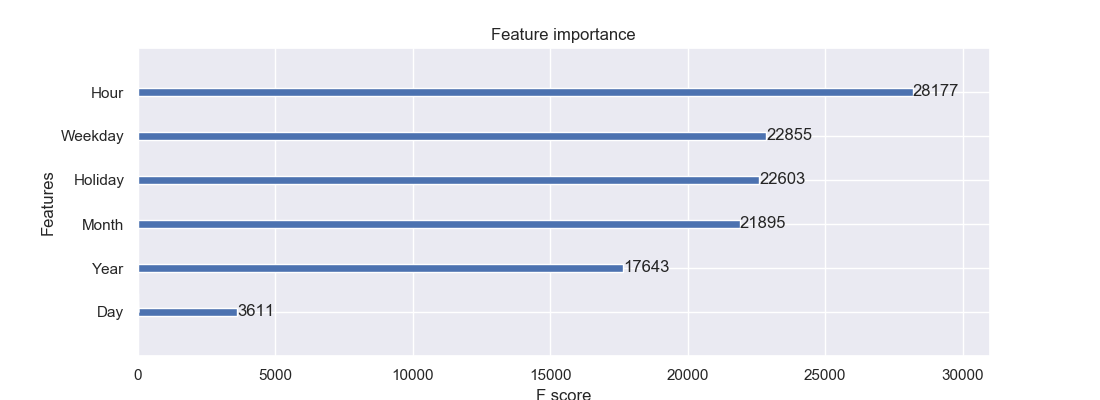
\includegraphics[width=1.0\textwidth,height=\textheight,keepaspectratio]{Figures/feature_importance_xgboost.png}
\caption{XGBoost Feature importance }
\label{figFeatImp2}
\end{figure}



\begin{figure}[!htpb]
\centering
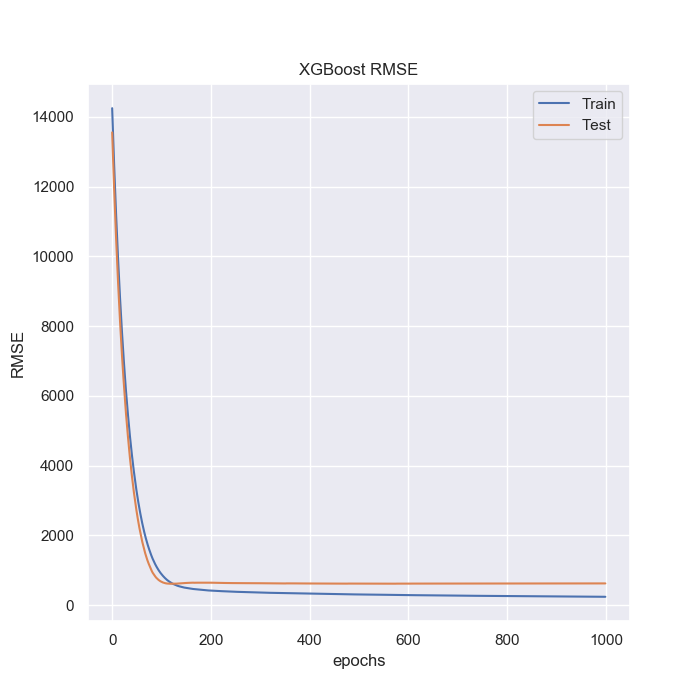
\includegraphics[width=1.0\textwidth,height=\textheight,keepaspectratio]{Figures/XGBoost_RMSE.png}
\caption{XGBoost - Root Mean Square Error (RMSE) curve}
\label{figXGBrmse}
\end{figure}


\begin{figure}[!htpb]
\centering
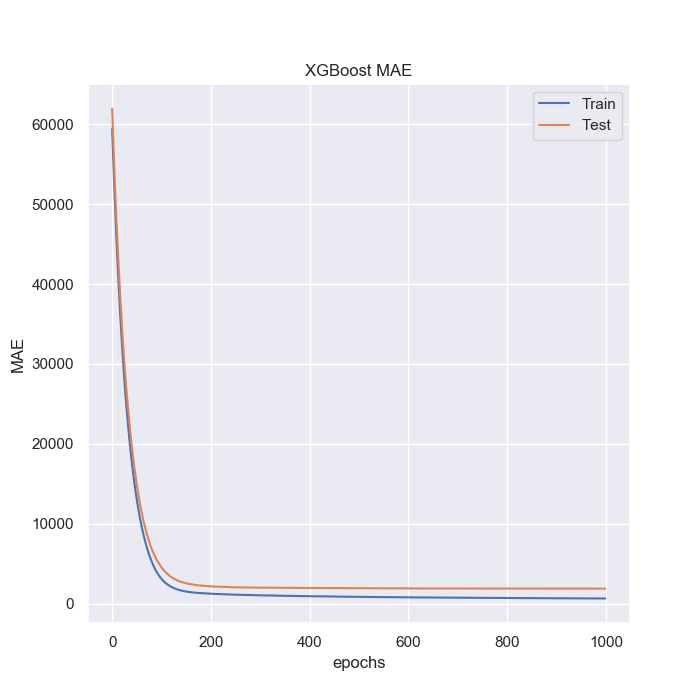
\includegraphics[width=1.0\textwidth,height=\textheight,keepaspectratio]{Figures/XGBoost_MAE.png}
\caption{XGBoost - Mean Average Error (MAE) curve}
\label{figXGBmae}
\end{figure}


\begin{figure}[!htpb]
\centering
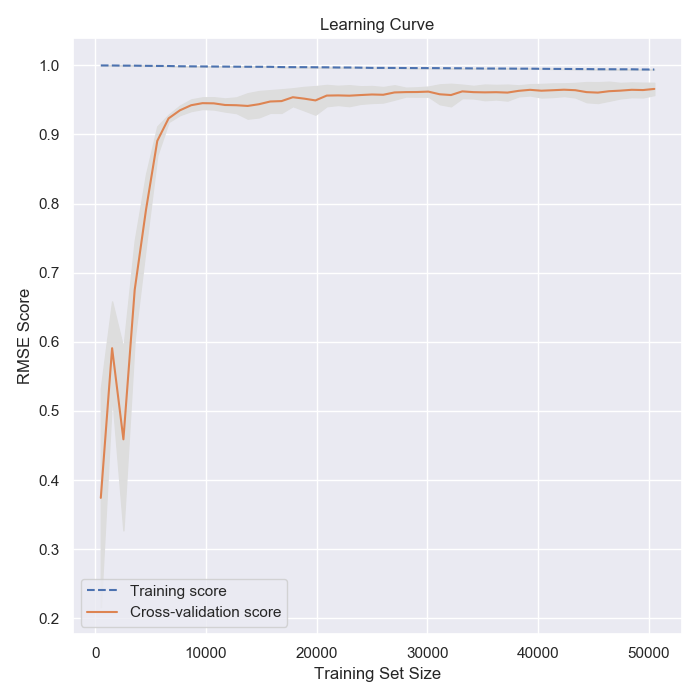
\includegraphics[width=1.0\textwidth,height=\textheight,keepaspectratio]{Figures/XGBoost_learningcurve.png}
\caption{XGBoost learning curve}
\label{figXGBlearn}
\end{figure}

